\documentclass[article]{jss}

%% -- LaTeX packages and custom commands ---------------------------------------

%% recommended packages
\usepackage{orcidlink,thumbpdf,lmodern}

\usepackage{amssymb}
\usepackage{amsmath}
\usepackage{siunitx}

%% another package (only for this demo article)
\usepackage{framed}

%% new custom commands
\newcommand{\class}[1]{`\code{#1}'}
\newcommand{\fct}[1]{\code{#1()}}


%% -- Article metainformation (author, title, ...) -----------------------------

%% - \author{} with primary affiliation (and optionally ORCID link)
%% - \Plainauthor{} without affiliations
%% - Separate authors by \And or \AND (in \author) or by comma (in \Plainauthor).
%% - \AND starts a new line, \And does not.
\author{Fernando Ferraz Ribeiro~\orcidlink{0000-0002-0685-4774}\\Universidade Federal da Bahia
   \And Gilney Figueira Zebende~\orcidlink{0000-0003-2420-9805}\\Universidade Estadual\\de Feira de Santana}
\Plainauthor{Fernando Ferraz Ribeiro, Gilney Figueira Zebende}
%  and $DMC_x^2$
%% - \title{} in title case
%% - \Plaintitle{} without LaTeX markup (if any)
%% - \Shorttitle{} with LaTeX markup (if any), used as running title
\title{A \proglang{Python}/\proglang{Zig} optimized and customizable implementation for the $\rho_{DCCA}$ and $DMC_x^2$ methods}
\Plaintitle{A Python/Zig optimized and customizable implementation for the Pdcca and DMCx2 methods}
\Shorttitle{\proglang{Python}/\proglang{Zig} implementation for the $\rho_{DCCA}$ and $DMC_x^2$}

%% - \Abstract{} almost as usual
\Abstract{
  This paper presents tha \pkg{Zebende}, a \proglang{Python} package written in \proglang{Python} and \proglang{Zig}, that calculates the $DFA$, $DCCA$ $\rho_{DCCA}$ and the $DMC_x^2$. The package presents an optimized algorithm that significantly improves the calculations speed. A comparison with other packages that calculates the $\rho_{DCCA}$. The package is also the first to implement the $DMC_x^2$ coefficient in a package and the first algorithm to calculates it for any number of time series.
}

%% - \Keywords{} with LaTeX markup, at least one required
%% - \Plainkeywords{} without LaTeX markup (if necessary)
%% - Should be comma-separated and in sentence case.
\Keywords{$\rho_{DCCA}$, $DMC_x^2$, optimization, \proglang{Python}, \proglang{Zig}}
\Plainkeywords{Pdcca, DMCx2, optimization, Python, Zig}

%% - \Address{} of at least one author
%% - May contain multiple affiliations for each author
%%   (in extra lines, separated by \emph{and}\\).
%% - May contain multiple authors for the same affiliation
%%   (in the same first line, separated by comma).
\Address{
  Fernando Ferraz Ribeiro\\
  Universidade Federal da Bahia\\
  Faculty of Achitecture\\
  Universit\"at Innsbruck\\
  Universit\"atsstr.~15\\
  6020 Innsbruck, Austria\\
  E-mail: \email{fernando.ribeiro@ufba.br}\\
  \emph{and}\\
  Centro Universitário Senai-Cimatec\\

  % URL: \url{https://www.zeileis.org/}
}

\begin{document}


%% -- Introduction -------------------------------------------------------------

%% - In principle "as usual".
%% - But should typically have some discussion of both _software_ and _methods_.
%% - Use \proglang{}, \pkg{}, and \code{} markup throughout the manuscript.
%% - If such markup is in (sub)section titles, a plain text version has to be
%%   added as well.
%% - All software mentioned should be properly \cite-d.
%% - All abbreviations should be introduced.
%% - Unless the expansions of abbreviations are proper names (like "Journal
%%   of Statistical Software" above) they should be in sentence case (like
%%   "generalized linear models" below).

\section{introduction} \label{sec:intro}

The Detrended Cross-correlation Coefficient ($\rho_{DCCA}$)~\citep{Zebende2011} is a widely used coefficient that measures the cross-correlation between two non-stationary time series. It´s an extension of the Detrended Fluctuation Analysis ($DFA$)~\citep{Peng_1994} and the Detrended Cross-correlation Analysis ($DCCA$)~\citep{Podobnik2008}: while the $DFA$ calculates the self-affinity and long-memory properties of a time series data, and the $DCCA$ analyses power-law cross correlations between two different non-stationary time series, the $\rho_{DCCA}$ coefficient quantifies this cross-correlation in simple values ranging from $-1$ to $1$, where $-1$ indicates a perfect anti-correlation between the series, $1$ a perfect correlation and zero ($0$) no correlation at all.

% rho DCCA applications

The Detrended Multiple Cross-Correlation Coefficient \citep{Zebende2018} ($DMC_x^2$) is a generalization of the $\rho_{DCCA}$ coefficient that correlates one time series (dependent variable) a number of time series (independent variables). The $DMC_x^2$ values ranges from zero ($0$), indicating no correlation to $1$, meaning perfect correlation or anti-correlation between the dependent and the independent variables.

% DMCx2 applications

This paper presents the \pkg{Zebende} \proglang{Python} package, an implementation of the $DFA$, $DCCA$, $\rho_{DCCCA}$, $DMC_x^2$ and utility functions related to the methods. In section \ref{sec:calculations} the steps for calculating the $\rho_{DCCCA}$ and $DMC_x^2$ are presented and discussed. Section \ref{sec:optimization} shows how this library was implemented, the optimization technics and the recommended steps to use the library. In Section \ref{sec:results} the \pkg{Zebende} package is compared with other packages for \proglang{Python} and \proglang{R} that calculates the $\rho_{DCCA}$ in terms of performance and usability, leading to the conclusions in Section \ref{sec:summary}.

\section{Algorithms of the coefficients}\label{sec:calculations}

The algorithms that calculates the $\rho_{DCCA}$ uses the $DFA$ and the $DCCA$ steps. The $DMC_x^2$ coefficient uses the $\rho_{DCCA}$ coefficient and, consequently, also embraces the $DFA$ and the $DCCA$. The $DFA$ method is described in six steps:


\begin{enumerate}\label{steps:dfa}

  \item Taking a time series $\{x_{i}\}$ with $i$ ranging from $1$ to $N$, the integrated series $X_{k}$ is calculated by $X_{k} = \sum_{i=1}^{k}\left[x_{i} - \langle x \rangle \right]$ with \(k\) also ranging from $1$ to $N$;
  \item the  $X_{k}$ series is divided in $N - n$ boxes of size $n$(time scale), each box containing $n + 1$ values, starting in $i$ up to $i + n$;
  \item for each box, a polynomial (usually of degree 1) best fit is calculated, getting $\widetilde{X}_{k, i}$ with $i \le k \le (i + n)$;
  \item in each box is calculated: $f_{DFA}^{2}(n, i) = \frac{1}{1+n} \sum_{k=i}^{i + n}(X_{k}-\widetilde{X}_{k})^{2}$
  \item for all the boxes of a time scale, the $DFA$ is calculated as:\\[10pt]
        $F_{DFA}(n) = \sqrt{\frac{1}{N - n} \sum_{i=1}^{N-n} f_{DFA}^{2}(n, i)}$;
  \item for a number of different timescales ($n$), with possible values $4 \le n \le \frac{N}{4}$ the $F_{DFA}$ function is calculated to find a relation among $F_{DFA} \times n$

\end{enumerate}


The $DCCA$ method is very similar to the $DFA$ calculations, with the difference of analyzing two series while the $DFA$ evaluate properties of a single time series. It´s also a six steps process:


\begin{enumerate}
  \label{steps:DCCA}
  \item Taking two time series with the same length $\{x\alpha_{i}\}$ and $\{x\beta_{i}\}$ with $i$ ranging from $1$ to $N$,
        the integrated series $X\alpha_{k}$ and $X\beta_{k}$ are calculated by
        $X_{k} = \sum_{i=1}^{k}\left[x_{i} - \langle x \rangle \right] $ for each series, with $k$ also ranging from $i$ to $N$;
  \item $X\alpha_{k}$ and $X\beta_{k}$ series are divided in $N - n$ boxes of size $n$(time scale), each box containing $n + 1$ values, starting in $i$ up to $i + n$;
  \item for each box, a polynomial (usually of degree 1) best fit is calculated, getting
        $\widetilde{X\alpha}_{k, i}$ and $\widetilde{X\beta}_{k, i}$,
        for series $\{x\alpha_{i}\}$ and $\{x\beta_{i}\}$ respectively,
        with $i \le k \le (i + n)$;
  \item in each box is calculated: $f_{DCCA}^{2}(n, i) =
          \frac{1}{1+n} \sum_{k=i}^{i + n}(X\alpha_{k}-\widetilde{X\alpha}_{k, i}) \times (X\beta_{k}-\widetilde{X\beta}_{k})$
  \item for all the boxes of a time scale, the $DCCA$ is calculated as:\\[10pt]
\end{enumerate}

Comparing the algorithms, the first three are basically identical, the only difference is that the $DCCA$ method apply those steps to two series. The step four of the $DFA$ can be considered an analogous of the variance, replacing the average subtraction (in the variance) for the values obtained by the polynomial fit (estimated series); and the equivalent step of the $DCCA$ is, in the same terms, compared to the covariance between the two series. The technique of fitting a curve, interpreted as a trend inside each box, and subtracting the value estimated by the trend from the actual value in the integrated series $(X_{k}-\widetilde{X}_{k})$ from now on will be called \textbf{detrended values}($DV$). In the $DFA$ algorithm, the $f_{DFA}^{2}(n, i)$ function is the mean of the square of the $DV$, in $DCCA$ calculations, the $f_{DCCA}^{2}(n, i)$ function evaluates the mean of the product of the $DV$ of the two series in each box.

Step five of the $DFA$ calculates the square root of the mean of the values calculates in the previous step for each box, in the $DCCA$, the mean of the values evaluated for each box is calculated in stead. The last step, in both cases, is more a reminder to repeat the respective previous operations for a number of difference time scales ($n$).

The $\rho_{DCCA}$ is measured using Eq. \ref{eq:p_dcca}. Considering the relation between $DFA$ and variance and $DCCA$ and covariance, the $\rho_{DCCA}$ resembles Pearson correlation for a time scale $n$.

\begin{equation}
  {\rho}_{DCCA}(n) = \frac{F_{DCCA~(x\alpha,~x\beta)}^{2}(n)}
  {F_{DFA~(x\alpha)}(n) \times F_{DFA~(x\beta)}(n)}
  \label{eq:p_dcca}
\end{equation}

The $DMC_x^2$ is a generalization of the $\rho_{DCCA}$ that calculates the correlation between one time-series $\left\lbrace Y \right\rbrace $, as the  dependent variable, and a number $j$ of time-series $\left\lbrace X_{1} \right\rbrace $, $\left\lbrace X_{2} \right\rbrace $, $\left\lbrace X_{3} \right\rbrace $, $\dots $, $\left\lbrace X_{j} \right\rbrace $ defined as independent variables. The coefficient is expressed mathematically as:

\begin{equation}
  {DMC}_{x}^{2}  \equiv \rho_{Y,X_{i}}(n)^{T} \times \rho^{-1}(n) \times \rho_{Y,X_{i}}(n)
  \label{eq:dmcx2}
\end{equation}

In Eq. \ref{eq:dmcx2}, $\rho^{-1}(n)$ represent the inverse of a matrix populated by all possible combinations of $\rho_{DCCA}$ between independent variables. In Eq. \ref{eq:p_dcca_matrix}, value $\rho_{X_{1},X_{2}}(n)$, for instance, is the $\rho_{DCCA}$ for independent variables $X_{1}$ and $X_{2}$ calculated with time scale $n$, occupying position $\rho_{1 2}$ of the matrix. Two fundamental characteristics: the first is that the main diagonal values are all ones, since it's position in the matrix denotes the calculation of a cross-correlation between a series and itself. Second, the matrix is symmetric in relation to the main diagonal, as the $\rho_{DCCA}$ is a commutative operation.

\begin{equation}
  \rho^{-1}(n) = \left(\begin{matrix}
    1                     & \rho_{X_{1},X_{2}}(n) & \rho_{X_{1},X_{3}}(n) & \dots & \rho_{X_{1},X_{j}}(n) \\
    \rho_{X_{2},X_{1}}(n) & 1                     & \rho_{X_{2},X_{3}}(n) & \dots & \rho_{X_{2},X_{j}}(n) \\
    \vdots                & \vdots                & \vdots                & \dots & \vdots                \\
    \rho_{X_{j},X_{1}}(n) & \rho_{X_{j},X_{2}}(n) & \rho_{X_{j},X_{3}}(n) & \dots & 1                     \\
  \end{matrix}\right)^{-1}
  \label{eq:p_dcca_matrix}
\end{equation}

At last Eq. \ref{eq:rhocol} represent the transposed vector of the $\rho_{Y,X_{i}}(n)$ between the depended variable $\left\lbrace Y \right\rbrace $ and each $\left\lbrace X_{i} \right\rbrace $ independent variable for a given time scale $n$.

\begin{equation} \label{eq:rhocol}
  \rho_{Y,X_i}(n)^T=[\rho_{Y,X_1}(n), \rho_{Y,X_2}(n),\cdots,\rho_{Y,X_j}(n)]
\end{equation}

As the $DFA$ and the $DCCA$,~$\rho_{DCCA}$ and~$DMC_x^2$ should be evaluated in a number of time scales ($n$) to analyze the characteristics of each coefficient.

%% -- Manuscript ---------------------------------------------------------------

%% - In principle "as usual" again.
%% - When using equations (e.g., {equation}, {eqnarray}, {align}, etc.
%%   avoid empty lines before and after the equation (which would signal a new
%%   paragraph.
%% - When describing longer chunks of code that are _not_ meant for execution
%%   (e.g., a function synopsis or list of arguments), the environment {Code}
%%   is recommended. Alternatively, a plain {verbatim} can also be used.
%%   (For executed code see the next section.)

\section{Zebende package: implementation and optimization} \label{sec:optimization}

The implementation of the \pkg{Zebende} package follows some well defined goals:

\begin{enumerate}
  \item Enhance performance;
  \item avoid redundant calculations;
  \item make the outputs compatibles with other data analyses tools (including data manipulation, machine learn and statistical packages);
  \item manage multiple time series inputs;
  \item operate the $DMC_x^2$ for any number of series;
  \item create a customizable and modular set of tools;
  \item facilitate package evolution and maintenance;
  \item deliver an easy to use package.
\end{enumerate}

The \proglang{Python} language was chosen because it´s one of the most used languages in the data analyses field and have a great support for statistical tools and machine learning algorithms. The are a plethora of tools to load and manipulate data (\pkg{Pandas}, \pkg{Polar}, \pkg{PySpark} ...), execute statistical analyzes (\pkg{Numpy}, \pkg{SciPy}, \pkg{StatsModels}~...), machine learning (\pkg{Pytorch}, \pkg{TensorFlow}, \pkg{Scykit Learn}~...) and data visualization(\pkg{Matplotlib}, \pkg{Seaborn}, \pkg{Plotly}~...) among other data related applications.

\begin{figure}[h!]
  \centering
  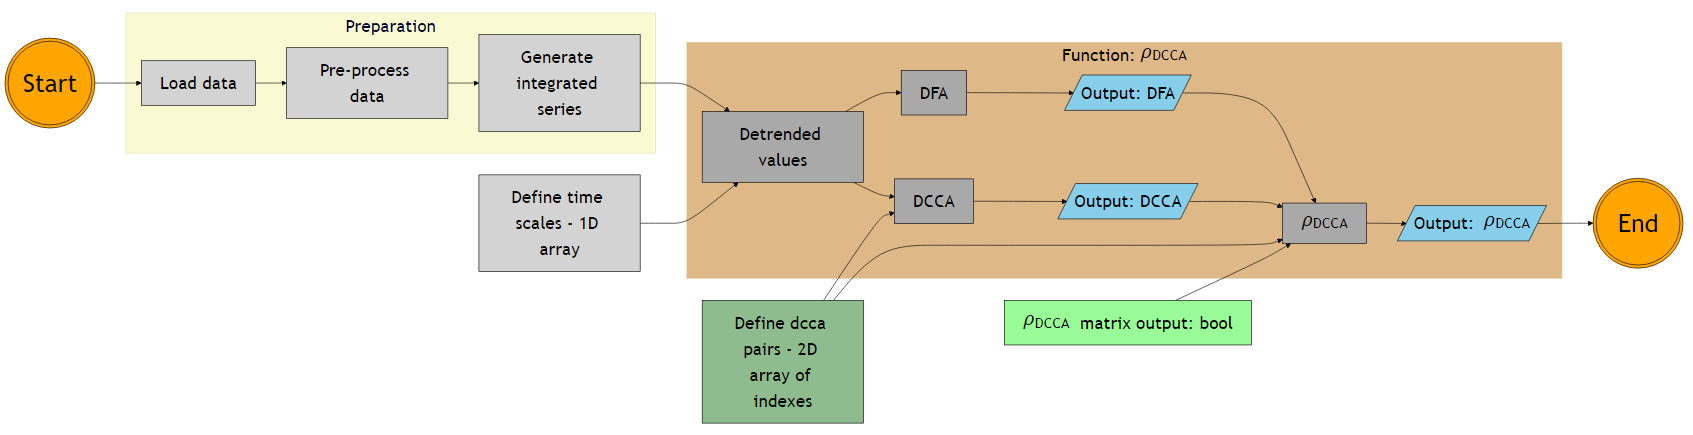
\includegraphics{./figs/pdcca_chart.png}
  \caption{\label{fig:pdcca_chart}Calculating  $\rho_{DCCA}$ with \pkg{Zebende} package - Simplified flowchart}
\end{figure}

The first draft of the code was written in pure \proglang{Python}, to rapidly prototype the way users will interact with the package. Figures \ref{fig:pdcca_chart} and \ref{fig:dmc_chart} presents simplified flowcharts illustrating how to use the package and how the main functions ($\rho_{DCCA}$ and $DMC_x^2$) works.

\begin{figure}[h!]
  \centering
  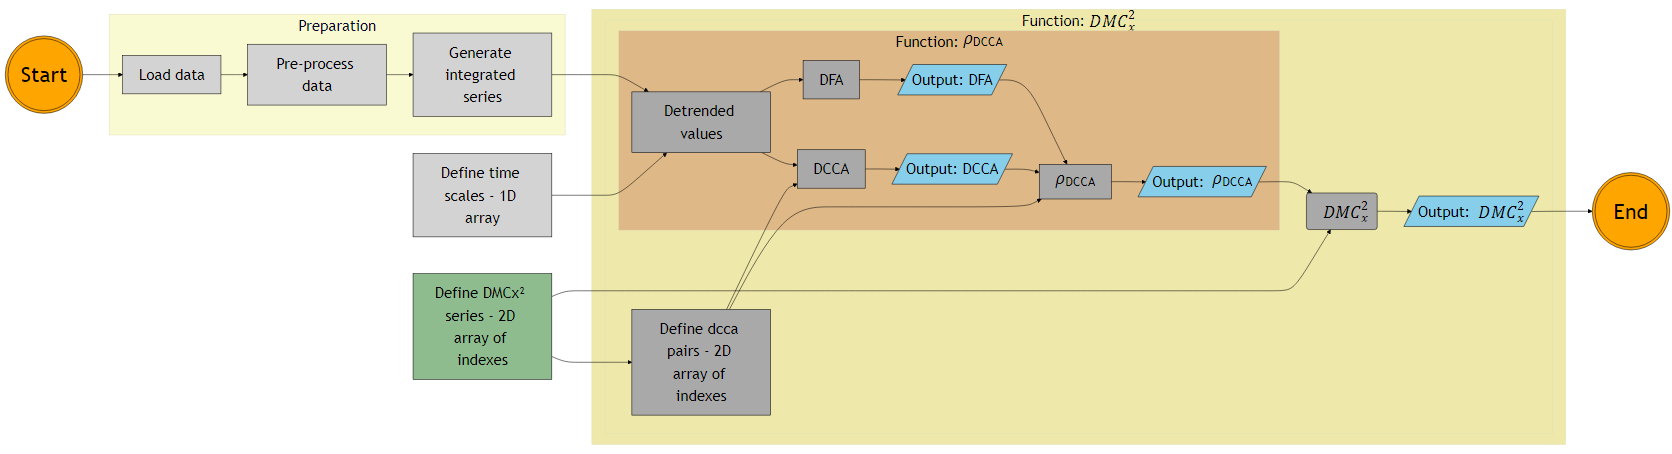
\includegraphics{./figs/dmc_chart.png}
  \caption{\label{fig:dmc_chart}Calculating  $DMC_x^2$ with \pkg{Zebende} package - Simplified flowchart}
\end{figure}

The preparation steps are the same in both functions. First the data is loaded, and should be analyzed by the researchers. Based on the data characteristics, the set should be treated to ensure the methods requirements in the "Pre-processing" stage. The package functions expects data as a matrix with the columns as the series and the lines as time steps. Columns unwanted in the indented research should also be dropped for better performance of the algorithms in this step. The more common way to do that is to use a data manipulation package. To proceed to the next step, the data table should be in the form of a \pkg{Numpy} 2D array. Any data manipulation \proglang{Python} package can export a table as a \pkg{Numpy} array. The next step is to calculate the integrated series. The package provides a function, named \verb"integrated_series()", to calculate that. The code example below show how to load the libraries (using \pkg{Pandas} as the data manipulation packages and loading a \verb".csv" file as a generic example), convert to \pkg{Numpy} array and generate the integrated series.

\begin{Code}
# importing packages
import numpy as np
import pandas as pd
import zebende as zb

data = pd.read_csv('path_to_the_file.csv') # loading data
# Pre-processing data
# ...
data = data.to_numpy(data) #converting data to Numpy array
int_data = zb.integrated_series(data) # calculating the integrated series
\end{Code}

The option of taking out the integrated series generation from the main methods (\verb"p_dcca()" and \verb"dmcx2()") to an independent one was inspired by \cite{Peng_1994} work, where the way of calculating integrated series was different from the one that is widely used in more recent years. The integration of the series is essentially a pre-processing step, and this approach makes easy to explore alternative ways to integrate the series or compare \cite{Peng_1994} approach to the current most used one in different scenarios, or even embrace new proposals for the series integrating step.

The input and output structures of each function are displayed below:

\begin{Code}
def p_dcca(
    input_data: NDArray[float64],
    tws: NDArray[int64] | NDArray[float64],
    DCCA_of: ndarray | Literal['all'] = "all",
    P_DCCA_output_matrix: bool = False
) -> tuple[NDArray[float64],  # DFA
          NDArray[float64],   # DCCA
          NDArray[float64]    # P_DCCA
          ]
\end{Code}

\begin{Code}
def dmcx2(
    input_data: NDArray[float64],
    tws: NDArray[int64] | NDArray[float64],
    dmcx2_of: ENUM_DMCx2_of | NDArray[float64] | list = 'all-full'
) -> tuple[ NDArray[float64],   # DFA
            NDArray[float64],   # DCCA
            NDArray[float64],   # P_DCCA
            NDArray[float64],   # DMC
          ]
  \end{Code}

The first two inputs are the same for functions \verb"p_dcca()" and \verb"dmcx2()": \verb"input_data" receive the integrated series and the \verb"tws" receives an 1D array representing the time scales (box size) described in the algorithms on Section \ref{sec:calculations}. The \verb"input_data" is a 2D array of 64 bits floating point data. The \verb"tws" accepts integers and, for convenience reasons, also floating points. Since the size of the boxes needs to be integers, in case of floating points, the values will be converted to integers by ignoring the decimal values (truncating). This two inputs are colored in light gray in Figures \ref{fig:pdcca_chart} and \ref{eq:dmcx2}, indicating mandatory inputs.

With the mandatory steps explained, some very important optional inputs should be addressed. Starting with the $\rho_{DCCA}$ function (dark green node in Figure \ref{fig:dmc_chart}) represents the input \verb"DCCA_of" of the function. This input requires a 2D array of integers, each row is a pair of index, related to the \verb"data_input" matrix. For example: if the \verb"input_data" receives a four columns matrix, with index ranging from $0$ to $3$, that is intended to calculate de $DFA$ for all the series but the $\rho_{DCCA}$ between series of index $0$ and $1$ and also for series $2$ and $3$, the \verb"DCCA_of" input should receive the array \verb"[[0,1], [2,3]]". If no value (or the string \verb"'all'") is given, the function will calculate all possible combinations of $DCCA$ calculations between all the series respecting the index values order, as below:

\begin{Code}
[[0,1], [0,2], [0,3], [1,2], [1,3], [2,3]]
\end{Code}

\subsection{Implementation of the Detrended Cross-correlation Coefficient function}

It´s important to understand the calculation steps, the role of the \verb"DCCA_of" array and how it fits in the goals of the package implementation. The code below is part of the pure \proglang{Python} implementation of the $\rho_{DCCA}$ function, 

\begin{Code}
for n_index, n  in enumerate(tws): # for each time scale
  # temporaty allocation arrays
  f2dfa_n = np.full(shape=(data.shape[0] - n, data.shape[1]),
  fill_value=np.nan, dtype=data.dtype)
  dcca_n = np.full(shape=(data.shape[0] - n, DCCA_of.shape[0]), 
  fill_value=np.nan, dtype=data.dtype)
  detrended_mat = np.full(shape=(n + 1, data.shape[1]), 
  fill_value=np.nan, dtype=data.dtype)
  for i in range(data.shape[0] - n): # for each box
      detrended_series( # inputs
                        time_steps[i : i + (n + 1)],  # arr_x
                        data[i : i + (n + 1), :],  # mat_y
                         detrended_mat,  # output
                      )
      f2dfa_n[i] = np.power(detrended_mat, 2).mean(axis=0)
      for j, pair in enumerate(DCCA_of): # for each DCCA pair
          dcca_n[i, j] = (detrended_mat[:, pair[0]] * detrended_mat[:, pair[1]]
                         ).mean(axis=0)
  F_DFA_arr[n_index, :] = np.sqrt(f2dfa_n.mean(axis=0))
  DCCA_arr[n_index, :] = dcca_n.mean(axis=0)
  # calculation of P_DCCA
  P_DCCA_output_function(n_index, DCCA_of, F_DFA_arr, DCCA_arr, # Inputs
  P_DCCA_arr) # Output
\end{Code}

The first \verb"for" loop in the code operates over the values of the \verb"tws" input, ensuring that step 6 of the $DFA$ and $DCCA$ methods, presented in Section \ref{sec:calculations}, is being carried out. In other words, the calculations will be applied, sequentially, to every single value in the \verb"tws" array. Three temporary arrays are allocated and resized for each time scale. The first, \verb"f2dfa_n", is used to store the calculations of the step 4 of the $DFA$~($f_{DFA}^{2}$). The number of lines of this array correspond to the number of boxes in the current time scale ($N - n$, resized for each time scale $n$) and the columns is the number of series in the analysis (same size for every value of $n$). Second, the array  \verb"dcca_n" holds the values calculated in the step 4 of the $DCCA$~(to calculate $f_{DCCA}^{2}(n, i)$). The number of lines also correspond to the number of boxes(resized for each $n$) but the number of columns equals the number of pairs (rows) in the \verb"DCCA_of" input (same size in each $n$). The \verb"detrended_mat" array has a number of lines equal to the number of points in a time scale box ($n +1$, resized for each $n$) and column count also equal to the number of time series (same size in each $n$). The first two temporary arrays will store data for all the boxes in the time scale, the last one will be used in each box and will have the values replaced in the next one, until the last box of the time scale. Than all the arrays will be cleared and recreated with shapes calculated with the new value of $n$.

After the allocation of the temporary arrays, the second \verb"for" loop operates in every box for a certain time scale $n$. In each box, the \verb"detrended_series()" function execute a one degree polynomial fit, subtract the values of the series with the value given by the interpolated curve($DV$) and stores this values in the \verb"detrended_mat". After that, the \textbf{mean of the square of each $DV$ in the box} ($f_{DFA}^{2}(n, i)$) is calculated in the current box for every time series and stored in the \verb"f2dfa_n" array in the line associated with the current box, and the column related to each time series.

The next nested \verb"for" loop operates over the \verb"DCCA_of" array. For each line (pair) in the \verb"DCCA_of" array, the $f_{DCCA}^{2}(n, i)$ is evaluated by multiplying the corresponding $DV$ from the two series  boxes in the current pair, getting the mean, and stores it in the \verb"dcca_n" temporary array.

After all the pairs are calculated, the algorithm goes back to the each box \verb"for" loop and head to the next box for the current time scale. when all the all the boxes are calculated, the final results for the $DFA$, $DCCA$ and $\rho_{DCCA}$ are evaluated and saved in the output vectors \verb"F_DFA_arr", \verb"DCCA_arr" and \verb"P_DCCA_arr" respectively.

The function named \verb"P_DCCA_output_function()" in the code above,is a pointer to other functions. One that outputs the  $\rho_{DCCA}$ results in the form of a table (rows for each time scale and columns for each \verb"DCCA_of" pair) and the other outputs it the form of a 3D matrix, where each level is the matrix in Equation \ref{eq:p_dcca_matrix} for one of the time scales. This behavior is driven by the \verb"P_DCCA_output_matrix" input (represented as the light green node in Figure \ref{fig:pdcca_chart}), where \verb"False" means table output and \verb"True" matrix output. This is very convenient for calculating the $DMC_x^2$. There are two utility functions to transform a table output in a matrix one (\verb"p_dcca_simple_to_matrix()") and also the other way around (\verb"p_dcca_matrix_to_simple()").

\subsection{Implementation of the Detrended Multiple Cross-correlation Coefficient function}

The \verb"dmcx2()" function runs the \verb"p_dcca()" with \verb"P_DCCA_output_matrix" set to \verb"True" in the background. There is no \verb"DCCA_of" input for the $DMC_x^2$ function, instead there is a \verb"dmcx2_of" parameter. This input receives a 2D matrix where each line represents the indexes of the series to be used in Equation \ref{eq:dmcx2}. For each row, the first elements is the index of the series used as the dependent variable, the others, the index of the independent ones. There are two literal strings that can be used, for convenience as inputs for this parameter: \verb"'all-full'", that generates a 2D array with every series as the dependent variable against all the others; and \verb"'first-full'", with only one row, having the index zero series as the dependent variable in relation with all the others. The \verb"'all-full'" option is conducted by calling \verb"dmc_of_all_as_y()", also available as a utility function.

With a given \verb"dmcx2_of" an array with all the necessary pairs for the $DCCA$ and $\rho_{DCCA}$ is automatically generated and used for the background \verb"p_dcca()" function to calculate da matrix as in Eq. \ref{eq:p_dcca_matrix}. The \verb"dcca_of_from_dmcx2_of()", also can be used as an utility function, receives the  \verb"dmcx2_of" as input and returns the \verb"dcca_of" array. With the matrix $\rho_{DCCA}$ assembled, two internal functions, that can also be used as utility functions, calculates the $DMc_{x}^2$ for all the lines in the \verb"dmcx2_of" matrix, for all the time scales. The first function, \verb"dmcx2_from_p_dcca_matrix()", that receives the $\rho_{DCCA}$ and the \verb"dmcx2_of" array, is presented in the code below.

\begin{Code}
def dmcx2_from_p_dcca_matrix(P_DCCA_arr: NDArray[np.float64], 
      dmcx2_of: NDArray[np.float64]) -> NDArray[np.float64]:   
    # DMCx2 output matrix
    DMCx2_arr = np.full(shape=(P_DCCA_arr.shape[2], dmcx2_of.shape[0]),
    fill_value=np.nan, dtype=P_DCCA_arr.dtype)

    for n_index in range(P_DCCA_arr.shape[2]):
        P_DCCA_arr_2D = P_DCCA_arr[:, :, n_index]
        for j,  dmcx2_of_1D in enumerate(dmcx2_of):
            DMCx2_arr[n_index, j] = dmcx2_from_p_dcca_matrix_2d(P_DCCA_arr_2D,
                                                                dmcx2_of_1D)
    return DMCx2_arr
\end{Code}

The \verb"dmcx2_from_p_dcca_matrix()" function executes a for loop over the $\rho_{DCCA}$ that separates the this 3D matrix in to the 2D matrices for each time scale. Nested in this loop, another \verb"for" extracts each line of the \verb"dmcx2_of" and passes, the extracted matrix and the line vector to the \verb"dmcx2_from_p_dcca_matrix_2d()", displayed here.

\begin{Code}
def dmcx2_from_p_dcca_matrix_2d(P_DCCA_arr_2D: NDArray[np.float64], 
          dmcx2_of_1D: NDArray[np.float64]) -> NDArray[np.float64]:   
  y_index = dmcx2_of_1D[0:1]
  x_indexes = dmcx2_of_1D[1:]

  mat_x = P_DCCA_arr_2D[np.ix_(x_indexes, x_indexes)]
  vec_y = P_DCCA_arr_2D[np.ix_(x_indexes, y_index)]

  return vec_y.T @ np.linalg.inv(mat_x) @ vec_y
\end{Code}

The \verb"dmcx2_from_p_dcca_matrix_2d()" function uses \pkg{Numpy} methods to prepare the data to apply Eq. \ref{eq:dmcx2}. The list of indexes is divided in \verb"y_index", holding an one item array whit the index of the dependent variable time series, and \verb"x_indexes", containing the indexes of the independent ones. The \pkg{Numpy} \verb"np.ix_()", although  it's not a very known function of the library constructs index arrays that will use the cross product from a series of 1D arrays as inputs. It's a very convenient way to extract a sub matrix and a vector from the $\rho_{DCCA}$ matrix. The matrix, as assembled by the \verb"p_dcca()" function, will always need to have extractions of a 2D matrix and a vector, as we can see in Eq.~\ref{eq:dmcx2}. The code below is an example of the extraction process.

\begin{CodeChunk}
\begin{CodeInput}
import numpy as np
arr = np.array([[1,2,3,4],
                [2,1,5,6],
                [3,5,1,7],
                [4,6,7,1]])
print(arr)
\end{CodeInput}

\begin{CodeOutput}
[[1 2 3 4]
 [2 1 5 6]
 [3 5 1 7]
 [4 6 7 1]]
\end{CodeOutput}
\end{CodeChunk}
An illustrative \verb"arr" matrix is defined as $4 \times 4$ with all ones in the main diagonal and symmetric integer values in the other cells. Since the $\rho_{DCCA}$ ranges from $-1$ to $1$, those values should be interpreted as place holders. 
\begin{CodeChunk}
\begin{CodeInput}
sub_mat_index = np.ix_([1,2,3], [1,2,3])
print("index combination:\n", sub_mat_index)
print("extracted matrix:\n",arr[sub_mat_index])
\end{CodeInput}

\begin{CodeOutput}
index combination:
(array([[1],
      [2],
      [3]]), array([[1, 2, 3]]))
extracted matrix:
[[1 5 6]
[5 1 7]
[6 7 1]]
\end{CodeOutput}
\end{CodeChunk}

Above, a sub matrix, holding the positions $1$ to $3$ is extracted using \verb"np.ix_()" function, and below, the extraction of the vector, first as a line and then as a column vector.
\begin{CodeChunk}

\begin{CodeInput}
sub_mat_vec = np.ix_([0], [1,2,3])
print("line vector:\n", arr[sub_mat_vec])
sub_mat_vec = np.ix_([1,2,3],[0])
print("column vector:\n", arr[sub_mat_vec])
\end{CodeInput}

\begin{CodeOutput}
line vector:
[[2 3 4]]
column vector:
[[2]
[3]
[4]]
\end{CodeOutput}
\end{CodeChunk}

In the \pkg{Zebende} package, the vector is extracted as a column for better coherence with the $DMC_{x}^{2}$ theory. The method also works for dependent variable different of index $0$. The resulting matrix will preserve the diagonal as $1$, the symmetry regarding the main diagonal and the order of elements in the column vector respected. the code below extract the index $1$ series as the dependent and the others as independent.
\begin{CodeChunk}
\begin{CodeInput}
sub_mat_index = np.ix_([0,2,3], [0,2,3])
print("index combination:\n", sub_mat_index)
print("extracted matrix:\n",arr[sub_mat_index])
sub_mat_vec = np.ix_([0,2,3],[1])
print("column vector:\n", arr[sub_mat_vec])
\end{CodeInput}

\begin{CodeOutput}
index combination:
(array([[0],
      [2],
      [3]]), array([[0, 2, 3]]))
extracted matrix:
[[1 3 4]
[3 1 7]
[4 7 1]]
column vector:
[[2]
[5]
[6]]
\end{CodeOutput}
\end{CodeChunk}

The idea of separating the calculations of the $\rho{DCCA}$ calculations in three distinct functions aims to different workflows. The \verb"dmcx2()" function calculates and outputs all the prerequisites, as the $DFA$, $DCCA$, $\rho_{DCCA}$ along with the $DMC_{x}^{2}$. This is the most practical way of getting all this calculations conducted. But the task can also be divided in two: first use the \verb"p_dcca()" function to generate $DFA$, $DCCA$, $\rho_{DCCA}$ outputs, analyze the outputs and then get the $DMC_{x}^{2}$ using \verb"dmcx2_from_p_dcca_matrix()".

Function \verb"dmcx2_from_p_dcca_matrix_2d()" can be used to more customizable applications. Imagine a use case where only the $\rho_{DCCA}$ anti-correlation, inside a certain range, in relation to the dependent variable, with the \verb"dmcx2_0f" set to \verb"all-full". From previous $\rho_{DCCA}$ studies is known that this coefficient can vary from positive to negative and vice  versa in different time scales. This implies that the $\rho_{DCCA}$ matrix should be analyzed in every time scale from every line of the \verb"dmcx2_of", also implies that the \verb"dmcx2_of" may not be a matrix in the since that the rows may have different. The \pkg{Numpy} ND Array could not hold that. Many different workarounds could be proposed for that situation. In the implementation of this package, function \verb"dmcx2_from_p_dcca_matrix_2d()" allow the user to make a custom code that extracts the  $\rho_{DCCA}$ matrix for the current time scale and extracts the elements that fit the rules from each \verb"dmcx2_of" row.

\subsection{Zig implementation}

The \proglang{Python} implementation successfully reflects the implementation goals presented in Sec.~\ref{sec:optimization} but the performance could benefit with the integration of a low-level language. \proglang{Zig} was chosen to enhance the algorithms performance. It's a low-level language that gain popularity in recent years and provides performance similar to \proglang{C} and \proglang{Fortran} in some scenarios~\citep{10820804}.

The interest for using \proglang{ZIg} for this project also relies on the cross-compiling capabilities of the \proglang{Zig} compiler. For a small research group maintaining a package could be challenging and the ability to to compile all releases for all platforms in a single machine is a great advantage. The \proglang{Zig} compiler can generate binaries for Windows, Linux and MacOS from a single machine. The \proglang{Zig} compiler is also very fast, and the language is very easy to learn, with a syntax that is very similar to \proglang{C}.

The implementation focus on writing technics $\rho_{DCCA}$ function in \proglang{Zig} exposed as a \proglang{C} Application Binary Interface (ABI), called by \proglang{Python} using the \pkg{ctypes} package. The $\rho_{DCCA}$ function is the most computational expensive part of the package, and the performance gain was expected to be significant.

The output arrays are allocated in the \proglang{Python} side and passed as pointers to the \proglang{Zig} function together with the series matrix, \verb"tws" and \verb"DCCA_of" arrays. The \proglang{Zig} function receives the pointers and the size of the arrays as inputs, and the results are stored in the same memory space. Before passing to \proglang{Zig} must be assured that the arrays are contiguous, using the \verb"np.ascontiguousarray()" function. The boolean parameter \verb"P_dcca_matrix_output" is also passed to the \proglang{Zig} function, to determine if the output of the $\rho_{DCCA}$ should be a table or a matrix.

The \proglang{Zig} implementation follows the same steps as the \proglang{Python} one, but repspecting languages differences. In \proglang{Python}, using \pkg{Numpy}, all the time series calculations occur in the same line of code, using the \pkg{Numpy} broadcasting capabilities. In \proglang{Zig}, the calculations are made in a nested \verb"for" loop.

\subsection{Algorithm optimization}

Although the \proglang{Zig} implementation presents a significant performance gain, the algorithm still can be optimized. The strategy is to focus on avoiding repeated calculations in the process. The code below shows the calculations of the polynomial fit before the optimization.

\begin{Code}
  pub fn lin_ls_fit(win: []f64, time: []f64) [2]f64 {
    var x_sum: f64 = 0;
    var y_sum: f64 = 0;
    var xy_sum: f64 = 0;
    var x2_sum: f64 = 0;
    for (win, time) |w, t| {
        x_sum += t;
        y_sum += w;
        xy_sum += t * w;
        x2_sum += pow(f64, t, 2);
    }
    const n: f64 = @as(f64, @floatFromInt(time.len));
    //slope
    const slope: f64 = (((n * xy_sum) - (x_sum * y_sum)) /
        ((n * x2_sum) - (pow(f64, x_sum, 2))));
    //inter
    const inter: f64 = ((y_sum - (slope * x_sum)) /
        (n));
    //result
    return [_]f64{ slope, inter };
}
\end{Code}

The code above calculates the slope and the intercept of a linear least squares fit. The function runs on every box for every time scale.In the optimized version, for consecutive boxes, the value of the sums from the previous box is used to calculate the next one without a loop for every item in the box.

\begin{equation}
  \label{eq:sum_opt_x}
  \forall~1<i\leq(N-n),~\sum_{k=i}^{i + n}T_k = \left(\sum_{j=i-1}^{(i+n)-1}T_j\right)~-~T_{i-1}~+~T_{i + n}
\end{equation}

\begin{equation}
  \label{eq:sum_opt_x2}
  \forall~1<i\leq(N-n),~\sum_{k=i}^{i + n}T_k^2 = \left(\sum_{j=i-1}^{(i+n)-1}T_j^2\right)~-~T_{i-1}^2~+~T_{i + n}^2
\end{equation}

\begin{equation}
  \label{eq:sum_opt_y}
  \forall~1<i\leq(N-n),~\sum_{k=i}^{i + n}S_k = \left(\sum_{j=i-1}^{(i+n)-1}S_j\right)~-~S_{i-1}~+~S_{i + n}
\end{equation}

\begin{equation}
  \label{eq:sum_opt_xy}
  \forall~1<i\leq(N-n),~\sum_{k=i}^{i + n} (S_k\times T_k) = \left(\sum_{j=i-1}^{(i+n)-1}(S_j \times T_j)\right)-(S_{i-1} \times T_{i-1})+(S_{i + n} \times T_{i + n})
\end{equation}

The expression in Eq.~\ref{eq:sum_opt_y} stands that the sum of the values in a box is equal to the sum of the previous box minus the first value of the previous box plus the last value of the current box. According to that, the 
when a box is calculated, the sum and the first value is saved in temporary variables, to calculate the next sum, the previous sum is subtracted from the temporary variable and the new value is added. The bigger the box, the bigger the gain in performance.

Also, to optimize the calculations from one time scale to the next, the first sums for the first box are saved in a temporary variable. Considering the current time scale as $tws_prev$ and the consecutive as $tws_current$. To calculate the current value, the algorithm takes the sums from the $tws_prev$ and add the values with indexes that exceed the $tws_prev$ size. The code was also rewritten with structs, to hold the temporary values and the functions for better readability. The code below shows the optimized version of polynomial fitting calculations.

\begin{Code}

fn shiftWindow( self: *MainOperator,
                n: usize, win_start: usize,
                F_DFA_ptr: *allowzero [*c]f64) void {
    self.time_window = self.time[win_start ..][ .. (n + 1)];
    // print("win_start {}\n", .{win_start});
    if (win_start != 0) {
        // updating sum_x
        self.current.sum_x = self.current.sum_x - self.left_x + self.time_window[n];
        // updating sum x^2
        self.current.sum_x2 = self.current.sum_x2 - 
        pow(f64, self.left_x, 2) + pow(f64, self.time_window[n], 2);
        // updating y and y*x for every serie
        for (self.series, 0..) |serie, sr_index| {
            serie.current.sum_y = serie.current.sum_y - 
            serie.left_y + serie.serie[win_start + n];

            serie.current.sum_xy = serie.current.sum_xy - 
            (self.left_x * serie.left_y) + 
            (self.time_window[n] * serie.serie[win_start + n]);
            serie.left_y = serie.serie[win_start];
            self.detrended(serie, win_start, &F_DFA_ptr.*[sr_index]);
        }
    } else { // win_start == 0
        self.current.window_len = n + 1;

        for (self.previous.window_len..self.current.window_len) |i| {
            self.previous.sum_x += self.time_window[i];
            self.previous.sum_x2 += pow(f64, self.time_window[i], 2);

            for (self.series) |serie| {
                serie.previous.sum_y += serie.serie[i];
                serie.previous.sum_xy += self.time_window[i] * serie.serie[i];
            }
        }

        // updating current sum values
        self.current.sum_x = self.previous.sum_x;
        self.current.sum_x2 = self.previous.sum_x2;

        for (self.series, 0..) |serie, sr_index| {
            serie.current.sum_xy = serie.previous.sum_xy;
            serie.current.sum_y = serie.previous.sum_y;

            serie.left_y = serie.serie[win_start];
            self.detrended(serie, win_start, &F_DFA_ptr.*[sr_index]);
        }
    }
    self.left_x = self.time_window[0];
}
\end{Code}
In the code above, the \verb"MainOperator" is a structure that holds the time series(y), the time window, the sums and the temporary values. The \verb"shiftWindow()" function is a method of the \verb"MainOperator" structure. The function receives the size of the box, the index of the first element of the box, and a pointer to the $F_{DFA}^{2}$ array. The function is called for every box in every time scale. The function is responsible for updating the sums of the time series, the sums of the $DV$ and the $DV$ matrix.

The three implementations, pure \proglang{Python}, \proglang{ZIg} and optimized \proglang{Zig}, where tested and the results are presented in the next section.
 
%% -- Illustrations ------------------------------------------------------------

%% - Virtually all JSS manuscripts list source code along with the generated
%%   output. The style files provide dedicated environments for this.
%% - In R, the environments {Sinput} and {Soutput} - as produced by Sweave() or
%%   or knitr using the render_sweave() hook - are used (without the need to
%%   load Sweave.sty).
%% - Equivalently, {CodeInput} and {CodeOutput} can be used.
%% - The code input should use "the usual" command prompt in the respective
%%   software system.
%% - For R code, the prompt "R> " should be used with "+  " as the
%%   continuation prompt.
%% - Comments within the code chunks should be avoided - these should be made
%%   within the regular LaTeX text.

\section{Results} \label{sec:results}




%% -- Summary/conclusions/discussion -------------------------------------------

\section{Summary and discussion} \label{sec:summary}


%% -- Optional special unnumbered sections -------------------------------------

% \section*{Computational details}

% \begin{leftbar}
%   If necessary or useful, information about certain computational details
%   such as version numbers, operating systems, or compilers could be included
%   in an unnumbered section. Also, auxiliary packages (say, for visualizations,
%   maps, tables, \dots) that are not cited in the main text can be credited here.
% \end{leftbar}

% The results in this paper were obtained using
% \proglang{R}~3.4.1 with the
% \pkg{MASS}~7.3.47 package. \proglang{R} itself
% and all packages used are available from the Comprehensive
% \proglang{R} Archive Network (CRAN) at
% \url{https://CRAN.R-project.org/}.


% \section*{Acknowledgments}

% \begin{leftbar}
%   All acknowledgments (note the AE spelling) should be collected in this
%   unnumbered section before the references. It may contain the usual information
%   about funding and feedback from colleagues/reviewers/etc. Furthermore,
%   information such as relative contributions of the authors may be added here
%   (if any).
% \end{leftbar}


%% -- Bibliography -------------------------------------------------------------
%% - References need to be provided in a .bib BibTeX database.
%% - All references should be made with \cite, \citet, \citep, \citealp etc.
%%   (and never hard-coded). See the FAQ for details.
%% - JSS-specific markup (\proglang, \pkg, \code) should be used in the .bib.
%% - Titles in the .bib should be in title case.
%% - DOIs should be included where available.

\bibliography{refs}


%% -- Appendix (if any) --------------------------------------------------------
%% - After the bibliography with page break.
%% - With proper section titles and _not_ just "Appendix".

% \newpage

% \begin{appendix}

%   \section{More technical details} \label{app:technical}

%   \begin{leftbar}
%     Appendices can be included after the bibliography (with a page break). Each
%     section within the appendix should have a proper section title (rather than
%     just \emph{Appendix}).

%     For more technical style details, please check out JSS's style FAQ at
%     \url{https://www.jstatsoft.org/pages/view/style#frequently-asked-questions}
%     which includes the following topics:
%     \begin{itemize}
%       \item Title vs.\ sentence case.
%       \item Graphics formatting.
%       \item Naming conventions.
%       \item Turning JSS manuscripts into \proglang{R} package vignettes.
%       \item Trouble shooting.
%       \item Many other potentially helpful details\dots
%     \end{itemize}
%   \end{leftbar}


%   \section[Using BibTeX]{Using \textsc{Bib}{\TeX}} \label{app:bibtex}

%   \begin{leftbar}
%     References need to be provided in a \textsc{Bib}{\TeX} file (\code{.bib}). All
%     references should be made with \verb|\cite|, \verb|\citet|, \verb|\citep|,
%     \verb|\citealp| etc.\ (and never hard-coded). This commands yield different
%     formats of author-year citations and allow to include additional details (e.g.,
%     pages, chapters, \dots) in brackets. In case you are not familiar with these
%     commands see the JSS style FAQ for details.

%     Cleaning up \textsc{Bib}{\TeX} files is a somewhat tedious task -- especially
%     when acquiring the entries automatically from mixed online sources. However,
%     it is important that informations are complete and presented in a consistent
%     style to avoid confusions. JSS requires the following format.
%     \begin{itemize}
%       \item JSS-specific markup (\verb|\proglang|, \verb|\pkg|, \verb|\code|) should
%             be used in the references.
%       \item Titles should be in title case.
%       \item Journal titles should not be abbreviated and in title case.
%       \item DOIs should be included where available.
%       \item Software should be properly cited as well. For \proglang{R} packages
%             \code{citation("pkgname")} typically provides a good starting point.
%     \end{itemize}
%   \end{leftbar}

% \end{appendix}

%% -----------------------------------------------------------------------------


\end{document}
